\documentclass[a4paper,10pt,oneside,openany]{jsbook}
\renewcommand{\figurename}{Fig.}
\renewcommand{\tablename}{Table.}
\bibliographystyle{junsrt}  % 電子情報通信学会の論文誌スタイルになってる
\usepackage{amsmath,amssymb}
\usepackage{bm}
\usepackage{cite}
% \usepackage{epsbox}  %図表貼りつけ関連.epsファイルを扱う
\usepackage[dvipdfmx]{graphicx}
\usepackage[dvipdfmx]{color}
\usepackage{verbatim}
\usepackage{wrapfig}
\usepackage{ascmac}
\usepackage{makeidx}
\usepackage{here}
\usepackage{subfigure}
%subcaption ON
\usepackage[hang,small,bf]{caption}
%\usepackage[subrefformat=parens]{subcaption}
%\captionsetup{compatibility=false}
%tableに色つけ
\usepackage{colortbl}
%図とかの位置 H
\usepackage{here}
%\usepackage{subfigure}

% セクション、サブセクションの文字の大きさ
\makeatletter
\def\@makechapterhead#1{
\vspace*{2\Cvs}
{\parindent \z@ \raggedright \normalfont
\Huge\headfont
\ifnum \c@secnumdepth >\m@ne
\if@mainmatter
\@chapapp\thechapter\@chappos
\hskip1zw
\fi
\fi
#1\par\nobreak
\vskip 3\Cvs}}
\makeatother

\makeindex
% 余白・文字数調整(左30mm, 右20mm, 上下共30mm, 文字数約40字/行, 行数約32行)
\setlength{\textwidth}{160truemm}      % テキスト幅: 210-(30+20)=160mm
\setlength{\fullwidth}{\textwidth}     % ページ全体の幅
\setlength{\oddsidemargin}{30truemm}   % 左余白
\addtolength{\oddsidemargin}{-1truein} % 左位置デフォルトから-1inch
\setlength{\topmargin}{30truemm}       % 上余白
\setlength{\textheight}{237truemm}     % テキスト高さ: 297-(30+30)=237mm
\addtolength{\topmargin}{-1truein}     % 上位置デフォルトから-1inch
\makeatother
\begin{document}
% タイトル設定
%\include{title}
\frontmatter
% 論文要旨
%\thispagestyle{empty}
\begin{center}
	{\large 東京農工大学 工学府 情報工学専攻 2018年度 修士論文 要旨}\\
	\vspace{8mm}
	{\Large 題目 手指使用量の常時計測のためのウェアラブルデバイスの開発}\\
	\vspace{2mm}
	{\large A wearable device for continuous monitoring of fingers activity}\\
	\vspace{8mm}
	{\large 学籍番号 17646137  氏名 松本 崇斗 (Takato MATSUMOTO)}\\
	\vspace{2mm}
	{\large 提出日 2018年1月30日}\\
	\vspace{4mm}
\end{center}














% 目次
\tableofcontents

\mainmatter

%!TEX root = _thesis.tex
\chapter{序論}

\section{はじめに}
脳卒中麻痺リハビリテーションの目標は,食事,更衣,入浴などの日常生活動作ができるように患者の麻痺肢機能を改善することである.麻痺肢機能の改善を促進する介入方法の有効性を評価するためには,介入後の日常生活において,患者の麻痺肢使用量が実際に増えたか否かについて,リハビリテーションの効果を定量的に測る手法が必要である.しかしながら,病院やリハビリ施設で実施する検査では,質問紙やヒアリングによる調査が主体であり,日常生活における麻痺肢使用量を正確に評価することができない.さらに,診療所や研究所で行われるテストでは,日常生活上での患者の麻痺肢使用量を計測することができない.現在,日常生活上の麻痺肢使用量を測定する手法として,Accelerometryが一般的である.しかし,この手法は加速度センサを用いており,手指の使用量を正確に計測,評価することができない.そのため,本研究では日常生活において,麻痺患者の麻痺肢使用,特に,手指の使用量を計測,評価する手法を提案する.

\section{日常生活動作(Activities of Daily Living)}
日常生活動作(ADL)とは食事,更衣,入浴など,日常生活を営む上で不可欠な基本的な動作のことである.
日常生活動作の評価はリハビリテーションの分野で患者の機能障害や効果測定のため開発された.
麻痺患者の多くは,日常生活動作をするのに必要な,肢機能が健常者に比べ低い.
麻痺肢の使用が障害回復に効果がある\cite{Zeiler2017}.




\section{上肢機能評価結果を用いた臨床判断}
麻痺肢機能評価から導かれた結果は,臨床医が患者の麻痺肢機能を治療,回復させる計画を立てる際に,非常に重要である\cite{Lang2013}.加えて,臨床医が麻痺障害後の麻痺肢機能や,その障害の回復を予測する際,麻痺肢機能評価の結果を見て判断を行う.複数の疫学的なデータから麻痺の回復は,時間経過と関係があると示唆されており,最も障害の回復が見込める期間は
,障害が引き起こってから三カ月以内であると言われている.麻痺の早期の障害の度合いは,最終的な運動障害に関係しており,軽度の障害である場合は,短期間で障害が回復し,3$\sim$6週間前後で障害が完治する可能性が高い.


\section{診療所や研究所で行われる上肢機能の評価手法}

\subsection*{Action Research Arm Test}
Action Research Arm Testは片側不全麻痺の患者の上肢機能評価手法である
\cite{Hsieh2009,Lang2008,Lang2013,Lang2017,Nijland2010,VanDerPas2011,VanDerLee2004,Taub1998}.この手法は19項目を握る,把持,ピンチ,全身運動の四つのサブスケールに
分け評価する手法である.上肢機能は各項目ごと0から3の四段階で評価され,各項目の評価が3であり,合計評価が57である場合,健常者と同等の上肢機能であると評価される.
\begin{figure}[H]
\begin{center}
\begin{tabular}{cc}
\subfigure[ARAT Kit]{
\includegraphics[scale=0.3]{fig/ch1/ARAT_kit}
} &
\subfigure[ARAT Score Sheet]{
\includegraphics[scale=0.3]{fig/ch1/ARAT_SCORING}
} \\
\end{tabular}
\end{center}
   \caption{Action Research Arm Test}
\label{fig:ARAT}
\end{figure}


\subsection*{Box and Block Test}
Box and Block Test\cite{T.2005,Mathiowetz1985,Desrosiers1993,Lin2010}は実施が簡単かつ実施時間が短い上肢機能評価手法であり,ブロックの把持,移動,解放動作を評価する手法である.
被験者は,1分間で多くのブロックを箱から別の箱に移動させることを指示される.この手法では,上肢機能の能力を1分間に動かしたブロックの個数で評価する.
\begin{figure}[H]
  \centering
  \includegraphics[width=0.8\linewidth]{fig/ch1/babt}
  \caption{Block and Block Test}
  \label{fig:babt}
\end{figure}

\subsection*{Chedoke Arm and Hand Activity Inventory}
Chedoke Arm and Hand Activity Inventoryは腕,手の麻痺障害後の回復度合いを評価する指標である\cite{}.
両手の使用を必要とするタスク13項目により,評価を行う.項目ごとに1$\sim$7の7段階で評価され,1は7の25\%以下の腕,手のパフォーマンスを意味する.
よって,高いスコアは,高い,腕や手のパフォーマンスを示す.タスクを行う時間が患者への負担となる場合,この手法を短時間で実施する手法として,Chedoke Arm and Hand Activity Inventory-9,Chedoke Arm and Hand Activity Inventory-8やChedoke Arm and Hand Activity Inventory-7といった手法がある.

\subsection*{Nine-Hole Peg Test}
Nine-Hole Peg Testは手の器用さを測る簡単な手法である.被験者はペグをホールに刺し,刺した九つのペグを全て抜き取ることを指示される.テストの開始からペグを全て取り終えるまでの時間を計測し,その時間により,被験者の手の器用さを評価する.
\begin{figure}[H]
  \centering
  \includegraphics[width=0.8\linewidth]{fig/ch1/nhpt}{}
  \caption{Nine-Hole Peg Test}
  \label{fig:nhpt}
\end{figure}


\subsection*{Motor Activity Log}

片上肢麻痺患者の日常生活上での麻痺肢使用量を測る標準的手法としてMotor Activity Log(MAL)\cite{Taub2006,Uswatte2005,Uswatte2000}がある.MALは,医師が患者に対し,麻痺肢使用の量と質について直接問う,質問形式の手法であり,測定結果が患者の認知レベルによる影響や質問者の主観的影響を受ける問題がある.そのため,客観的な測定手法が必要である.MALの質問項目は,一般的な日常生活動作に関する質問である.日常生活動作とは,電気のスイッチをオンにする動作や引き出しを開ける動作といった,日常生活を営む上で最低限必要な動作である.MALの評価用紙をFig.\ref{fig:Motor Activity Log}に示す.MALの質問項目は30項目あり,日常生活動作時の麻痺肢使用の量と質について11段階の評価で患者が答える.

\begin{figure}[H]
\begin{center}
\subfigure[Score sheet]{
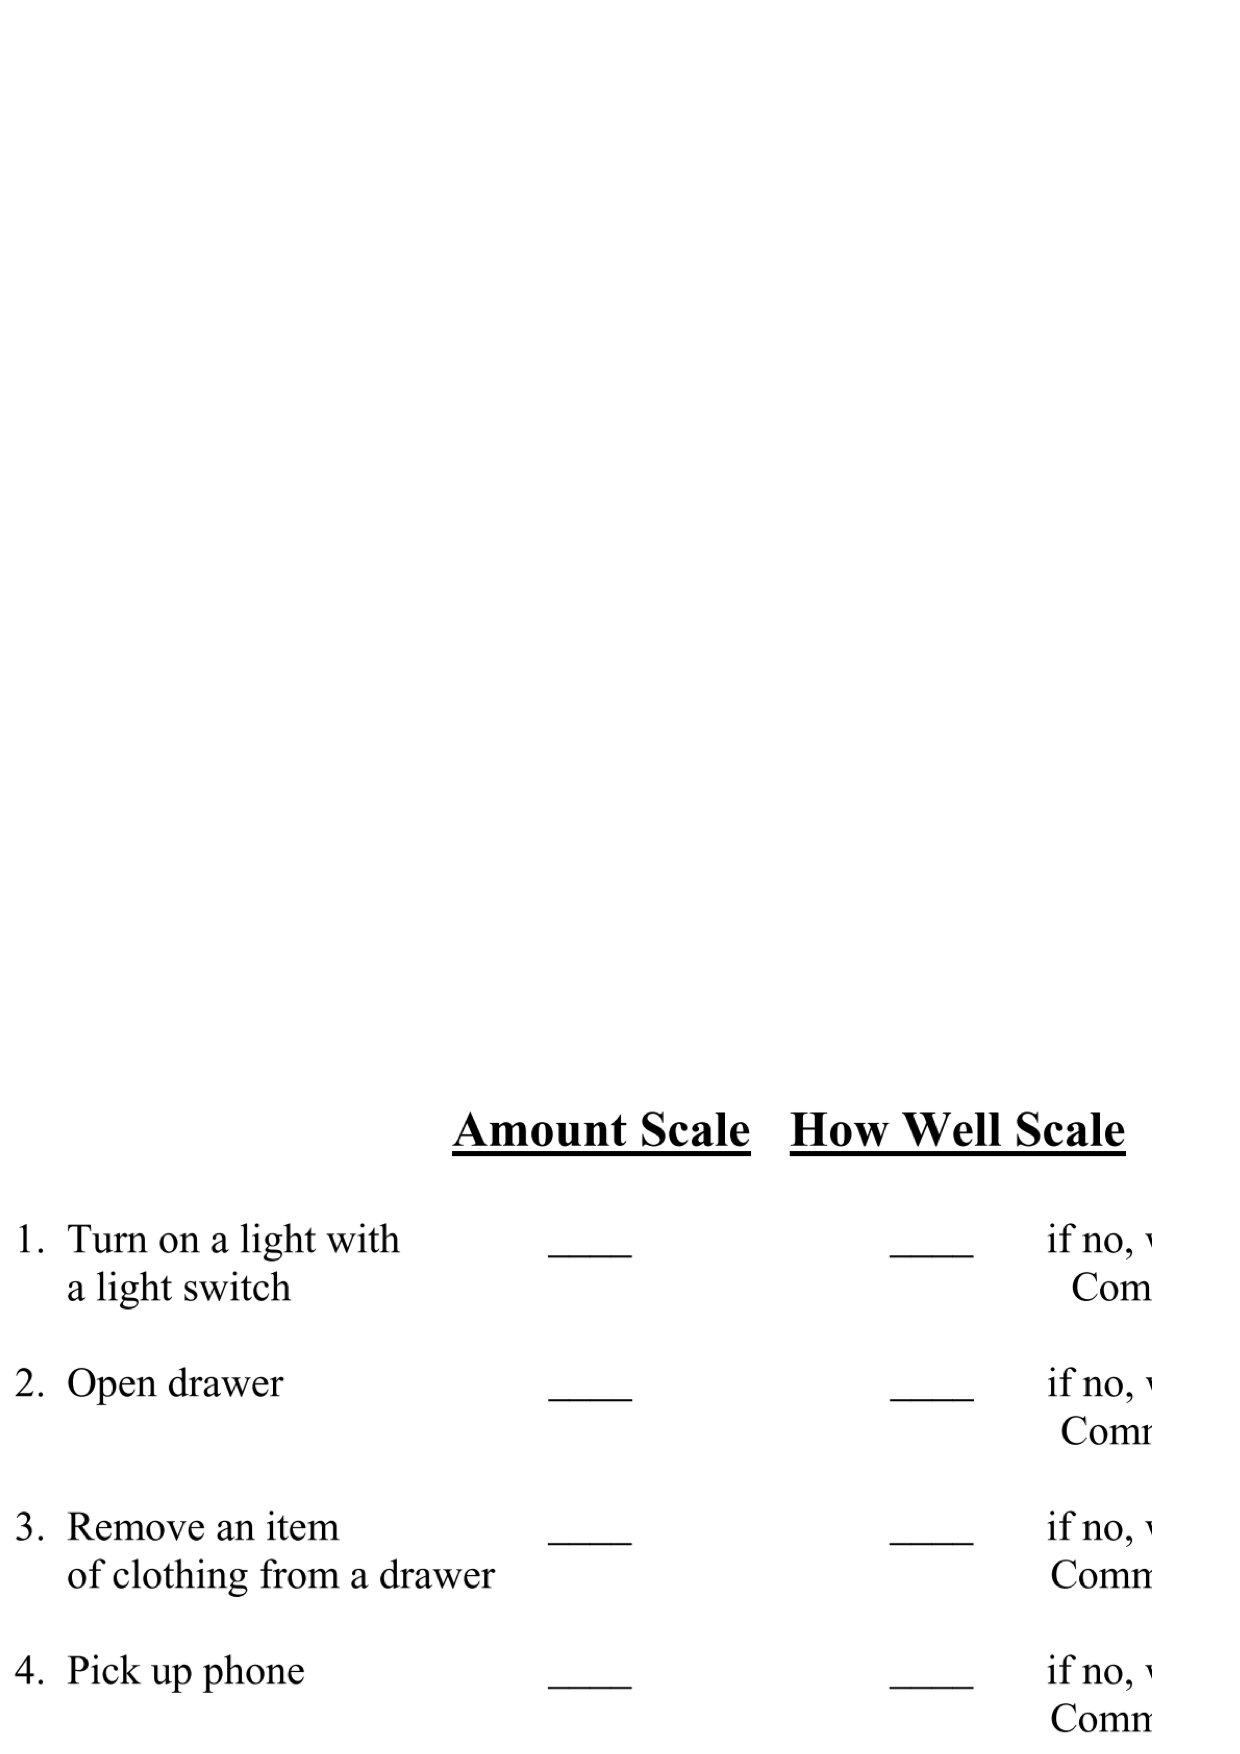
\includegraphics[scale=0.5]{fig/ch1/mal}
}
\begin{tabular}{cc}
\subfigure[Amout Scale]{
\includegraphics[scale=0.3]{fig/ch1/amount}
} &
\subfigure[How Well Scale]{
\includegraphics[scale=0.3]{fig/ch1/how}
} \\
\end{tabular}
\end{center}
   \caption{Motor Activity Log}
\label{fig:Motor Activity Log}
\end{figure}

\subsection*{Wolf Motor Function Test}
Wolf Motor Function Testは15個のタスクを含む上肢機能と患者の活動度合いを評価する手法である.1$\sim$6のタスクは関節の動きについて,7$\sim$15のタスクは総合的な上肢機能の評価項目である.患者は時間内にタスクをどれだけ遂行できたか(Functional Ability Score)で評価され,0はタスクを全く完了できないことを意味し,5はタスクを完全に完了できたことを意味する.時間での評価では,短い時間でタスクを完了できた場合,高い上肢機能であると評価する.

これらの手法は,患者の運動機能を計測,評価することが可能である.しかし,これらの手法は,定量的でない.また,日常生活上での患者の麻痺肢使用量を計測することができない.



\section{定量的上肢使用量計測に関する研究}
\subsection*{Accelerometry}
Accelerometry\cite{Chen2005,Hayward2016,Dwiputra2017,VanDerPas2011,VanDerLee2004,Thrane2011}をFig.\ref{fig:Accelerometry}に示す.Accelerometryは,加速度計が埋め込まれた腕時計型のウェアラブルデバイスで上肢の使用量を測る手法である.Accelerometryは麻痺肢の手首に装着することで,麻痺肢の使用量を測定する.データ記録装置とバッテリーが内蔵されているため,麻痺肢使用量の常時計測に向いている\cite{VanDerPas2011}.しかし,この手法で計測される加速度データはノイズを多く含み,信頼性の高いデータを得ることができない.加速度データに混入するノイズは,測定された加速度が所定の時間内に,閾値を超える場合にのみ,麻痺肢使用のスコアを増加するといった手法の閾値フィルタを用いて低減することができる.このアプローチによって得られたスコアは日常生活において,腕を動かした時間と高い相関を持つことが示されている.しかし,閾値フィルタを使用したノイズ低減を行った場合,加速度が閾値に達しない小さな手の動きが見落とされる可能性がある.また,加速度計が手首に装着されているため,手首や手の精密な動きを計測できない問題がある.これらの理由から,Accelerometryは指の使用量の測定には向かない\cite{Uswatte2000}.
また,Accelerometryはタスクを行なっているのか,歩行時に手を振っているのかということを見分けられない.歩行時に腕を振っていることを検知する手法があるが,この手法は,足やつま先などに追加のAccelerometryを装着することを必要とする\cite{Ullery2015}.
さらに,Accelerometryはどのタスクをしているのかを見分けることも難しい\cite{Hayward2016}.
\begin{figure}[H]
  \centering
  \includegraphics[width=0.8\linewidth]{fig/ch1/acc}
  \caption{Accelerometry}
  \label{fig:Accelerometry}
\end{figure}

Accelerometryの信頼性と妥当性




\subsection*{Data Glove}
Data gloveは手袋型のセンシング機器である.手袋の中に,曲げセンサまたは光ファイバーが内蔵されている.Data gloveは手全体を覆うセンサが存在しているため,センサによる指や手の動きの阻害や,
Data gloveの取り外しによる煩雑さ,水で手を洗えないといった問題がある.

\begin{figure}[H]
  \centering
  \includegraphics[width=0.6\linewidth]{fig/ch1/dataglove}
  \caption{Data glove}
  \label{fig:Data glove}
\end{figure}

\subsection*{Motion Capture System}
Motion capture systemはカメラ画像や赤外線距離センサによって,人体の動きをデジタルデータ取得するシステムである.手のモーショントラッキングに特化した,モーションキャプチャシステムにLeap MotionやUbiHand,Digits\cite{Ahmad2006,Kim2012}がある.これらの手法は赤外線カメラにより,手の動きをトラッキングするシステムである.しかし,精度の問題から指の動きといった小さな動きを取得するのは難しい.また,モーションキャプチャシステムを構成する計測機器を常に持ち運んで運用することは難しい.そのため,常に持ち運びができ,精度よく指のトラッキングが行えるシステムが必要である.

\begin{figure}[H]
  \centering
  \includegraphics[width=0.6\linewidth]{fig/ch1/mcs}
  \caption{Motion Capture System(Leap Motion)}
  \label{fig:Motion Capture System}
\end{figure}

\subsection*{Manumeter}
Manumeter\cite{Friedman2014}は磁力計と磁石の指輪を用いて手首や指の使用量を測定する手法である.ManumeterをFig.\ref{fig:Manumeter}に示す.手首に取り付けてあるデバイスは磁力計,加速度計とデータ記録のためのストレージ,マイクロコンピュータで構成されている.指の動きを磁石と磁力計間の磁力変化により推定し,指の使用量を測定する.本手法は指の使用量の測定精度が低いという問題点がある.
\begin{figure}[H]
  \centering
  \includegraphics[width=0.6\linewidth]{fig/ch1/manumeter}
  \caption{Manumeter}
  \label{fig:Manumeter}
\end{figure}

\subsection*{Behind The Palm}
手の甲の皮膚の皺をパターン認識することによって,指ジェスチャを識別するBehind The Palm\cite{Recognition2017}といった手法が発表されている.ャリブレーションによるユーザーへの負担が大きい,ジェスチャの認識ができるが,精確な手の動作の動きの認識ができないという問題がある.
\begin{figure}[H]
  \centering
  \includegraphics[width=0.6\linewidth]{fig/ch1/btp}
  \caption{Behind The Palm}
  \label{fig:Behind The Palm}
\end{figure}

研究レベルではData gloveやGoniometer,Motion capture system\cite{Binh2014,Valtin2017,Chen2003,Ren2011}などが手首や手の使用量を測定するために使用される.しかしながら,これらの手法は指の動きの阻害,空間的な制限といった問題があるため,日常生活における長時間の常時計測には向いていない.これらの理由から,依然として日常生活下の指の使用量を常時計測する手法は確立していない.本研究では,日常生活下の上肢片麻痺患者の麻痺肢使用,特に指の使用量を測る手法を提案し,手指使用量の常時測定のためのウェアラブルデバイスの開発を目的とする.


\section{本論文の構成}
本論文の構成を以下に記述する.第1章では本研究の背景と既存の研究について紹介する.第2章では,本研究で開発するデバイスの開発方法や,計測されたセンサデータの信号処理について記述する.第3章では,実験方法と結果を記述する.第4章では
実験によって得られた結果に対する考察と,本研究の課題を記述する.
%!TEX root = _thesis.tex
\chapter{手指使用量常時計測の理論と計測ステム構築}

\section{手指使用量の常時計測方法}
既存の手法の問題点を考察すると,手指使用量の常時計測に向いた計測手法は以下の要件を満たす必要がある.

\begin{itemize}
 \item 計測機器が持ち運びやすい
 \item ノイズに対してロバストである
 \item 定量的である
 \item ユーザへの負担が少ない
\end{itemize}

そのため,これらの要件を満たし,手指使用量が計測可能なウェアラブルデバイスの開発を目的とする.計測機器が持ち運びやすいを満たすには,軽量でコンパクトな計測機器が求められる.



\section{指の関節角度計測}
本研究の手指使用量の測定手法は,指の関節角度の変化が,指の使用量を反映するという仮定に基づく.関節角度の変化の推定には,ウェアラブルデバイスに搭載された赤外線距離センサを用いる.本デバイスは指の基節に装着して使用し,赤外線距離センサで,デバイスから中節までの距離を常時計測する.式(1)の関数を用い,測定された距離を指の関節角度に変換し,指の使用量を測る.距離を角度変換する模式図をFig.\ref{fig:principle}に示す.

\begin{figure}[H]
  \centering
  \includegraphics[width=0.8\linewidth]{fig/principle}
  \caption{Measurement principle}
  \label{fig:principle}
\end{figure}

\begin{equation}
\theta = \cos^{-1} \frac{x}{r}
\label{eq:theta}
\end{equation}


ここで,$r$は第二関節から指先までの長さ,$x$は最大屈曲時からの変化距離,$\theta$は最大伸展時からの変化角度である.
$r$はデバイス使用前に物差しやスケール等を用い測定しておく必要がある.$x$は本デバイスの赤外線距離センサによって測定,推定する.この$r,x$の二つのパラメータと式\ref{eq:theta}を用いることで,関節角度$\theta$を導出する.


\section{ウェアラブルデバイスのハードウェア}
本デバイスはLED(Osram SFH4550)とフォトトランジスタセンサ(Honeywell SD5410)で構成された赤外線距離センサを用いた指輪型のセンシング部と,手首に取り付けるデータ記録部から成るウェアラブルデバイスである.ウェアラブルデバイスをFig.\ref{fig:device}に示す.データ記録のため,マイコン基盤(Adafruit Faether M0)と32GBのSDcardを使用する.また,デバイスの電源として3.7V,400mAhのリポバッテリーを利用し,これにより24時間以上の連続電源供給が可能である.

さらに,マイコン基盤に三軸加速度センサ(KXR94-2050)を追加した.赤外線距離センサと加速度センサからの信号は,信号の入力時間とともにマイコン基盤に接続されたmicro sdカードへ保存される.PCへUSB2.0 A Male Microケーブルで接続することで,本デバイスのリポバッテリーの充電と,Micro sdカードに記録されたデータの転送が可能である.

本デバイスの指輪型の装着部分及び,バッテリーとマイコン基盤を収納するためのケースを3DCAD(Fusion 360)で設計し,3Dプリンタ(Dimension 1200es)で印刷し作成した.

\begin{figure}[H]
\begin{center}
\begin{tabular}{cc}
\subfigure[Hardware of the wearable device]{
\includegraphics[scale=0.3]{fig/fal6}
} &
\subfigure[Infrared distance sensor]{
\includegraphics[scale=0.3]{fig/fal7}
} \\
\subfigure[A LiPO battery]{
\includegraphics[scale=0.3]{fig/fal3}
} &
\subfigure[Micro SDcard and Accelerometer]{
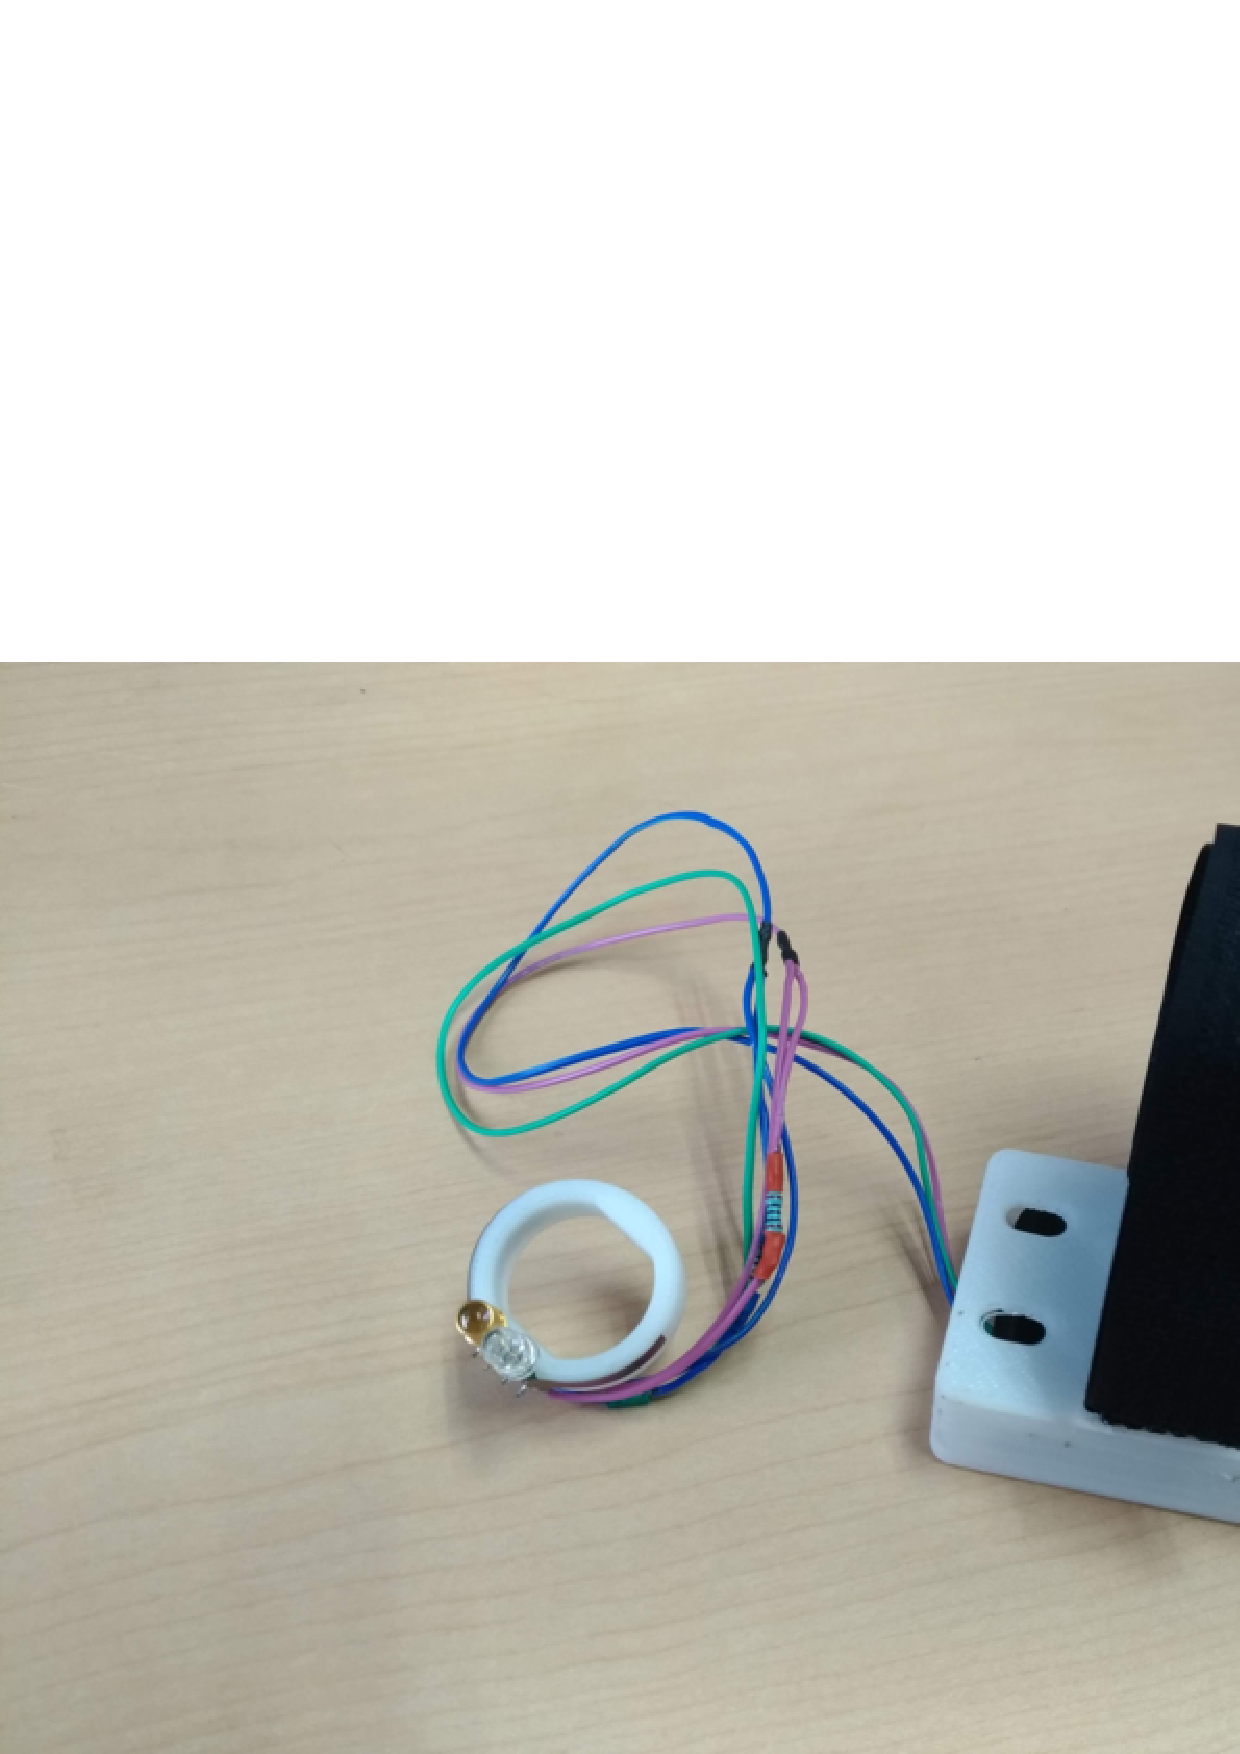
\includegraphics[scale=0.2]{fig/fal1}
} \\
\end{tabular}
\end{center}
\caption{Hardware}
\label{fig:device}
\end{figure}

\if0
(a)Hardware of wearable device.Sensing and data-logging board used to collect and store infrared distance sensor and accelerometry data.(b)Infrared distance sensor consists of LED and Phototransistor.
(c)A LiPO battery powers the unit for more than 24 hours and is recharged via a USB cable when attached to a computer.(d)Micro SDcard to store sensing-data and Accelerometer.
Fig.\ref{fig:device}の(a)は本デバイスのハードウェアを示したものである.センシング部と,データ記録部から構成され,赤外線距離センサと加速度センサのデータを記録する.(b)はLEDとフォトトランジスタで構成される赤外線距離センサを指輪に取り付けた,センシング部である.(c)は本デバイスに搭載されたリポバッテリーを示しており,このバッテリーにより24時間以上の連続計測と,USBケーブルを通じての充電が可能である.(d)はデータロギングボードに直接取り付けられた加速度センサと,データ記録用のMicro SDcardを示している.
\fi

本デバイスに取り付けられたスイッチをオンにすると,赤外線距離センサと加速度センサの記録を開始する.スイッチをオフにするまで連続計測,記録する.データはCSVファイルでSD card内に保存される.本デバイスに記録されたデータは,コンピュータと本デバイスのdeta-logging boardのArduinoをUSBケーブルで直接繋ぐか,Micro SDcardをコンピュータに移すことで,アクセスが可能である.

本デバイスの装着方法をFig\ref{fig:ring}に示す.指輪型のセンシング部は,食指の第二関節に装着し,ストレージ部は手首にマジックテープを使用し取り付ける.



\begin{figure}[h]
  \centering
  \includegraphics[width=0.8\linewidth]{fig/fal4.png}
  \caption{Ring worn on the index finger and Strage worn on the wrist}
  \label{fig:ring}
\end{figure}



\begin{figure}[H]
  \centering
  \includegraphics[width=0.5\linewidth]{fig/test}
  \caption{Circuit of the wearable device}
  \label{fig:circuit}
\end{figure}



\section{センシングキャリブレーション}
赤外線距離センサは物体に反射し,フォトトランジスタで受光した赤外線の強度を計測することで,距離を推定する.
しかし,同じ距離であっても赤外線が反射する物体によっては,違う
受光量となる場合がありえる.これは物体によって光の反射率が違い,同じ距離で計測したとしても,フォトトランジスタで受け取る受光量が違ってくるためである.つまり,人によって,指の長さや皮膚の色が違うため,同じセンサ値であっても,本来の距離が変わる問題がある.この問題を解決するために,被験者ごとに皮膚の反射率を調べることが望ましいが,本システムは日常生活での使用を目的としており,キャリブレーションがユーザに負荷をかけないことが求められる.
そのため,本システムでは計測される距離と受光量の関係を求め,キャリブレーションが可能な方法を提案する.キャリブレーションには以下の3つのパラメータを用いる.

\begin{itemize}
 \item デバイスを装着する指の長さ
 \item 指伸展時のセンサ情報
 \item 指屈曲時のセンサ情報
\end{itemize}

得られたセンサ情報と指の長さのデータにより,線形近似を行い,ユーザごとのキャリブレーションを行った.




\section{センシング情報の処理方法}
デバイスにより取得できる電圧値は,ノイズを含んでいるため,ノイズの除去を行った.
また,ノイズの除去はバターワイスローパスフィルターにより,10hz以上の周波数を持つシグナルをカットオフすることで行った.赤外線距離センサのセンシングデータから指間接角度を推定する際、いくつかの信号処理を行った.さらに、指の使用量へ変換する処理も行った.それら処理を以下に示す.

\begin{enumerate}
 \item 100Hzのサンプリングレートをもつセンシングデータを10Hzにダウンサンプリングした
 \item  ローパスフィルタにより、ノイズデータを除去した.1次元線形回帰により、センシングデータを,センサから指までの距離へ変換した.
 \item 関節角度が90度,0度のときのセンシングデータを利用し,キャリブレーションを行った
 \item 式\ref{eq:theta}により,距離を角度に変換した
 \item 角度を時間微分し,角度時間の変化角度を導出した
 \item 変化角度の絶対値をとり,タスクごとの指の使用量(タスクの合計変化角度)を導出した.
\end{enumerate}

%!TEX root = _thesis.tex
\chapter{精度評価手法と結果}

\section{指の長さ計測}
本デバイスのキャリブレーションには,ユーザの指の長さデータが必要である.そのため,ユーザの食指の第二関節から指先までの長さをメジャーを用い,計測した.実験の被験者の食指の第二関節から指先までの長さのデータを以下に示す.また,第二指長の計測結果を以下に示す.被験者は8名が男性,2名が女性である.

\begin{table}[H]
  \caption{Length between fingertip and proximal interphslangeal joint with index finger(n=10)}
  \label{table:finger_distance}
  \centering
  \begin{tabular}{ccc}
    \hline
    Subjects & Index finger& Between fingertip and proximal interphslangeal joint(cm)  \\
    \hline \hline
    A  & 2.71 & 0.993\\
    B  & 2.62 & 0.995\\
    C  & 6.61 & 0.985\\
    D  & 5.01 & 0.994\\
    E  & 2.33 & 0.995\\ 
    F  & 2.87 & 0.995\\
    G  & 1.57 & 0.998\\
    H  & 2.87 & 0.992\\
    I  & 3.04 & 0.986\\
    J  & 2.41 & 0.994\\
    \hline
  \end{tabular}
\end{table}

実験の被験者の食指の第二関節から指先までの長さの平均と標準偏差は,

また,第二指長の平均と標準偏差は




\section{ジェスチャ識別}
予備実験として健常者を対象に,本システムのジェスチャの認識精度を調査した.この実験の際は,LED(Osram SFH4550)とフォトトランジスタセンサ(Honeywell SD5410)の代わりに,赤外線距離センサ(Pololu QTR-1A)を2つ使用し,Fig.\ref{fig:sensor}の位置に取り付けた.

\begin{figure}[H]
  \centering
  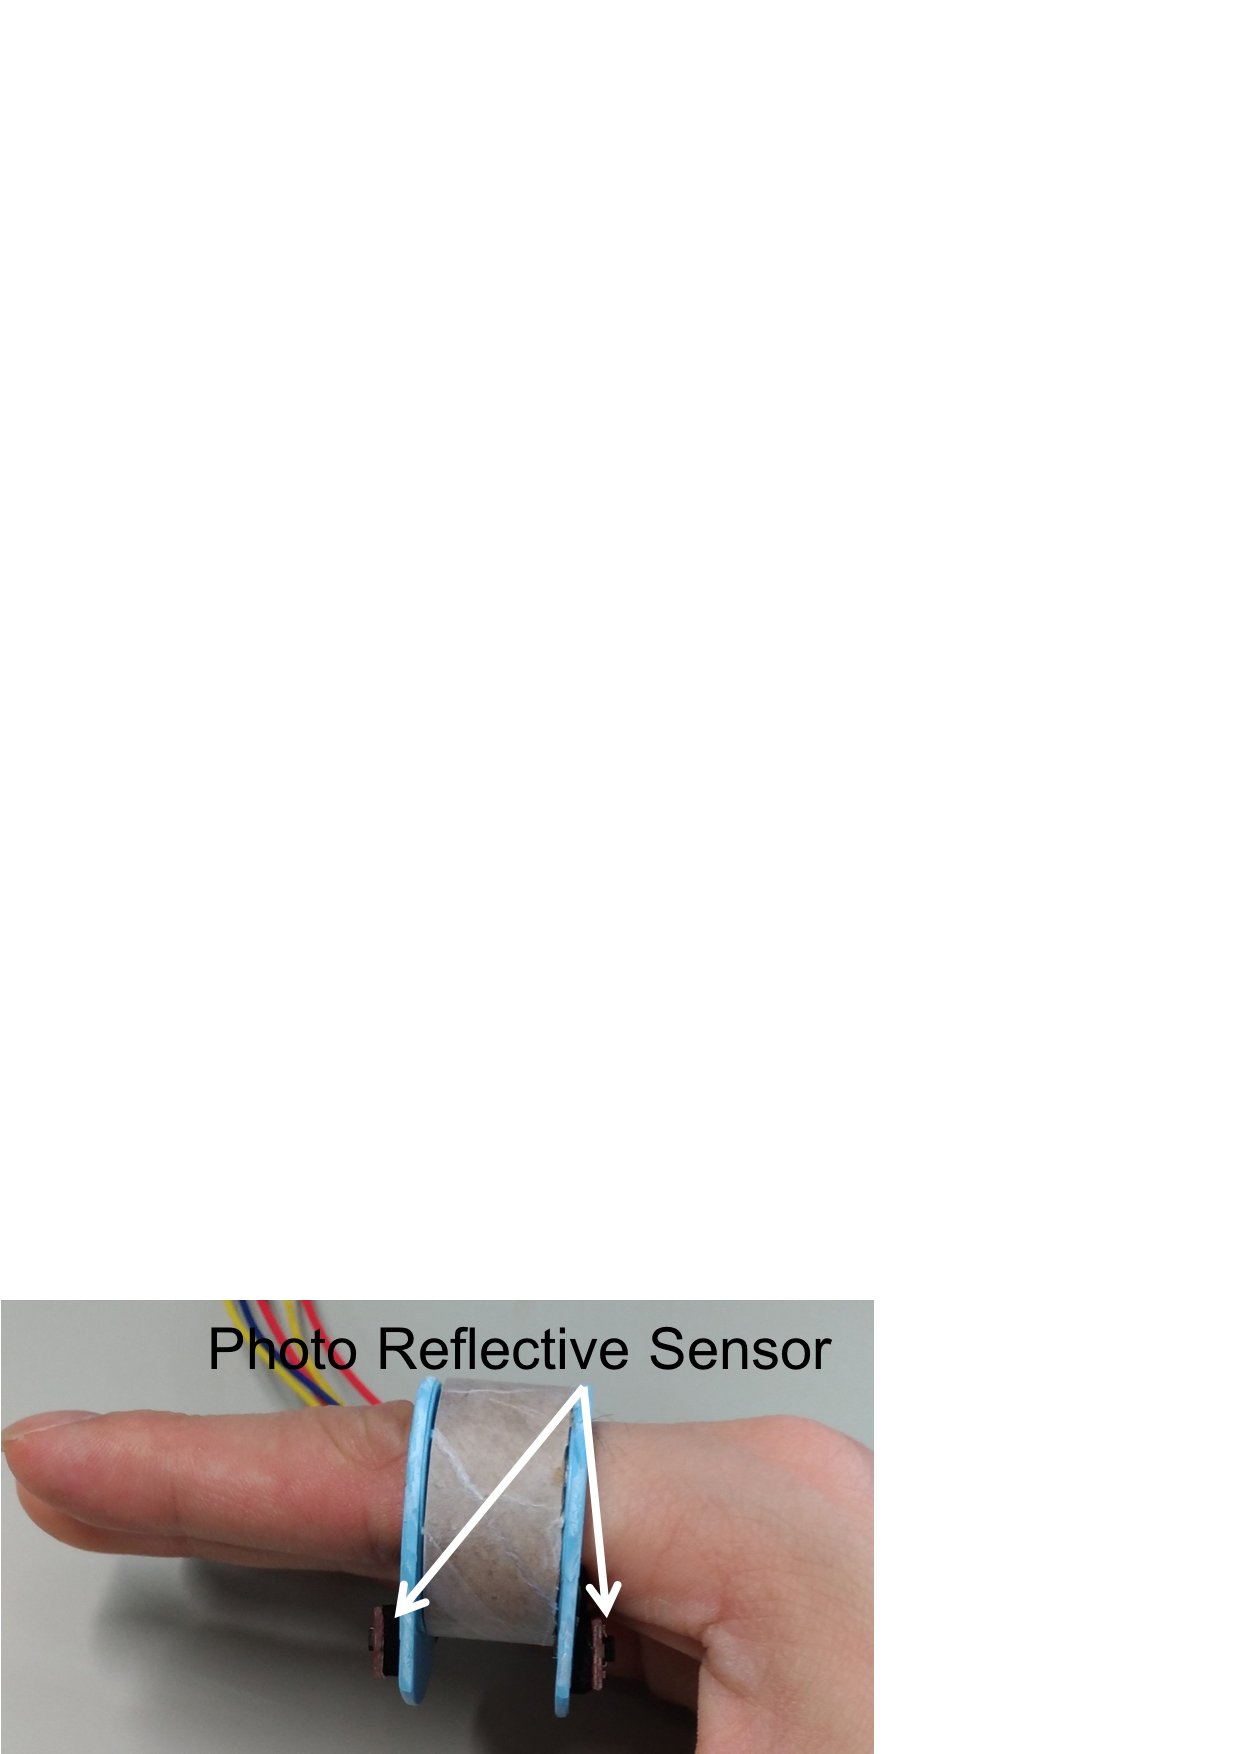
\includegraphics[width=0.6\linewidth]{fig/sensor}
  \caption{Mounting position of sensor}
  \label{fig:sensor}
\end{figure}

ジェスチャの種類をFig.\ref{fig:gesture}に示す.手指を閉じた状態(Fig.\ref{fig:gesture}の1),示指と母指で輪を作った状態(Fig.\ref{fig:gesture}の2),手指を開いた状態(Fig.\ref{fig:gesture}の3),計三つのジェスチャを指示し被験者に行ってもらった.これらのジェスチャは\cite{Lin2015}を元にした.被験者は椅子に座った状態で,本デバイスを装着した手でジェスチャを行った.一つのジェスチャを5秒間保持してもらい,その時のセンサーデータを収集した.
ジェスチャを5秒間保持している時の,センサ値の標準偏差は推定角度に変換すると被験者平均でSD=$\pm0.12度$であり,ごく小さいものだった.5秒間のセンサーデータを時間で平均したセンサ値をジェスチャ識別のために利用した.
また,センサデータは各ジェスチャにつき60回記録し,五人の被験者センサデータを収集した.センシングの際のサンプルレートは100\ Hzとした.
合計で一人につき180データ(60データ$\times$3ジェスチャ)を収集した.

\begin{figure}[H]
  \centering
  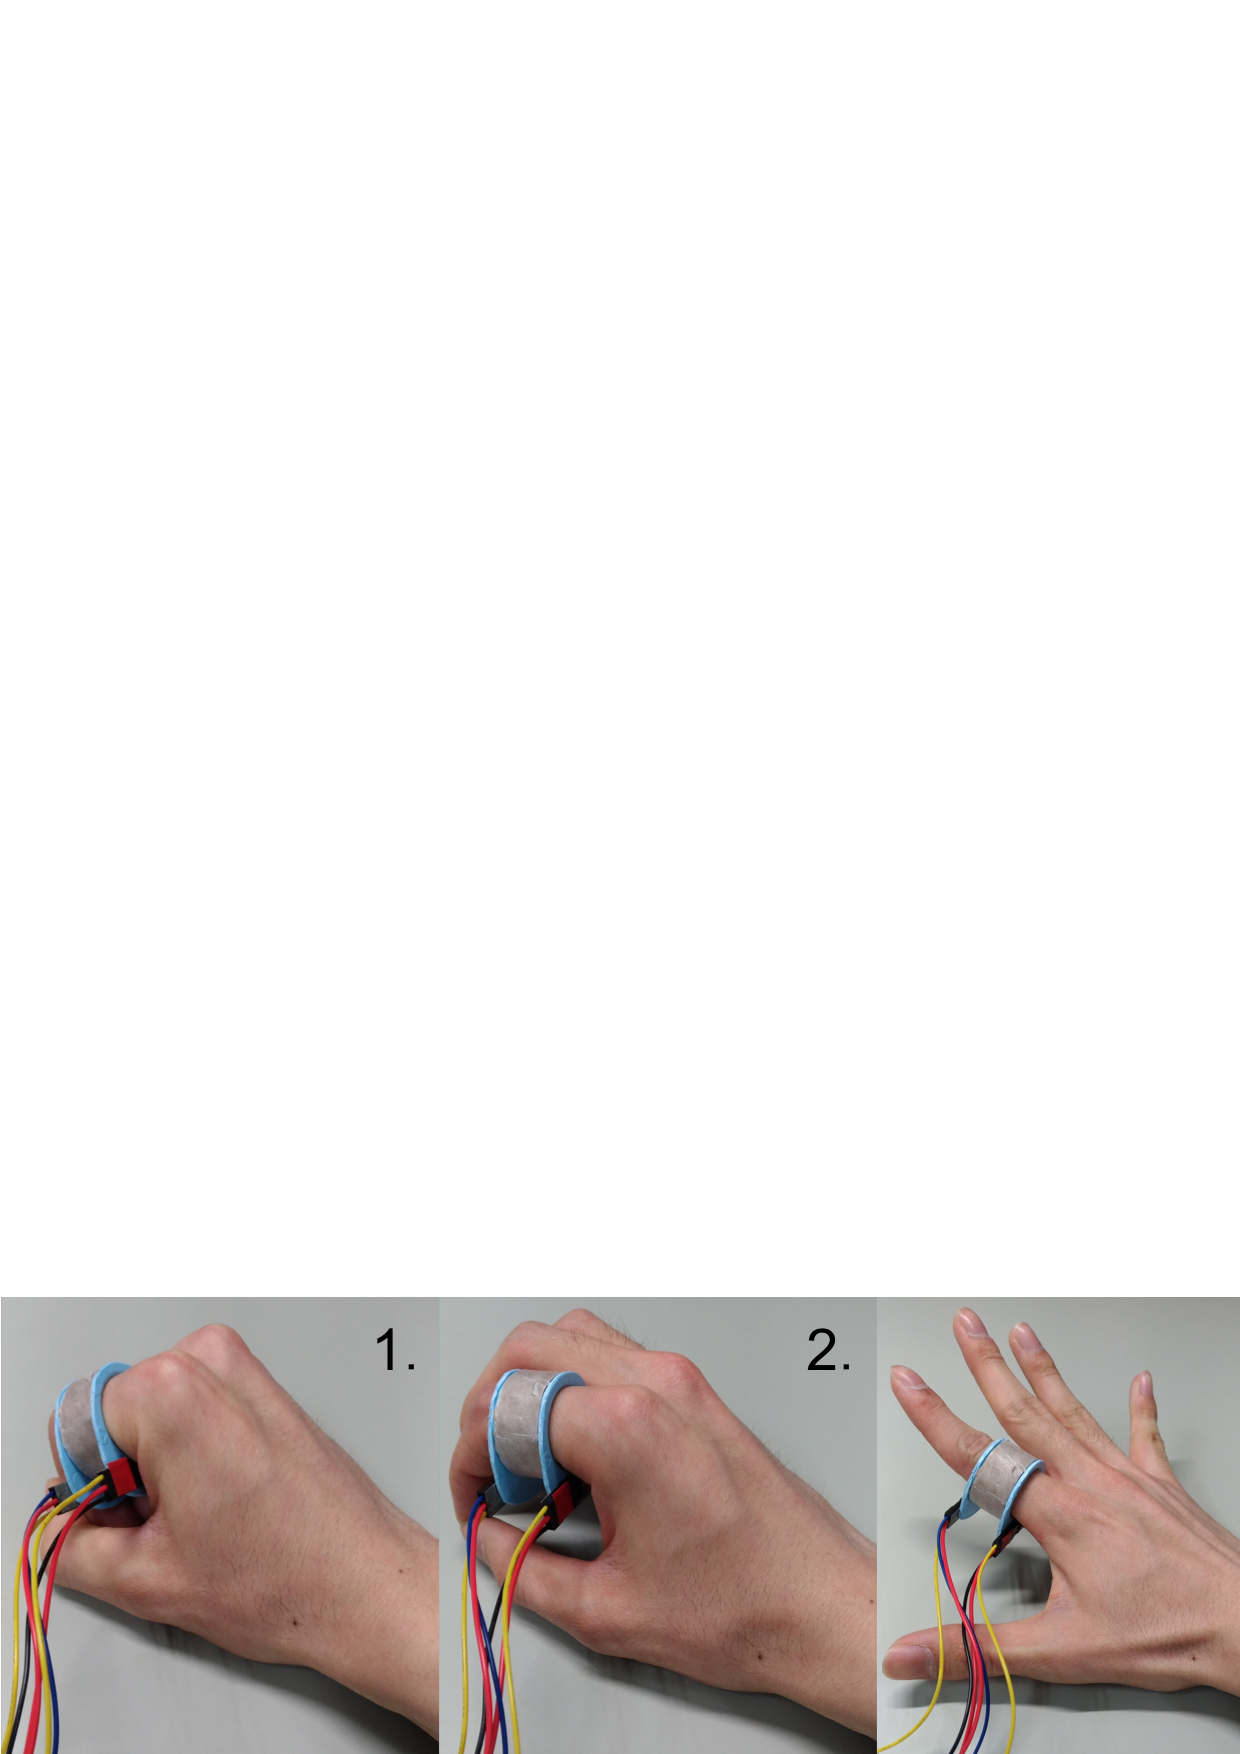
\includegraphics[width=0.8\linewidth]{fig/gesture}
  \caption{Prepared hand-gesture set}
  \label{fig:gesture}
\end{figure}

三つのジェスチャを識別するため,一対一分類法,線形Support Vector Machineを用いた.五人すべて,900データ(180データ$\times$五人)をジェスチャごとにラベル分けし,ジェスチャ識別に利用した.これらのデータの内,各ラベルに対し,データの80\%をトレーニングデータ,20\%をテストデータとした.

\begin{figure}[H]
  \centering
  \includegraphics[width=0.8\linewidth]{fig/confusion_matrix}
  \caption{Confusion matrix of 3-gesture}
  \label{fig:matrix}
\end{figure}


Fig.\ref{fig:matrix}より,ジェスチャ1と3を100\%の正解率で識別することが可能であることが分かった.五分割交差検証を行った結果,ジェスチャの平均正解率は98.9\%,分散3.9\%であった.この結果から本手法により三つのジェスチャの識別が可能であることが示された.



\section{関節角度推定}
健常者十人を対象に本デバイスの関節角度の推定精度の評価を行なった.被験者の指の関節を0$\sim$90°まで15°刻みで固定し,その時の関節角度の推定精度を評価した.指関節角度の固定には以下のFig\ref{fig:kotei}に示す器具を使用する.この器具は3DCAD(Fusion 360)で設計し,3Dプリンタ(Dimension 1200es)で印刷し作成した.この器具をFig.\ref{fig:kotei}(b)に示すとおり,食指の第二関節にあて関節角度を固定する.Fig.\ref{fig:kotei}(b)では$45^\circ$に固定されている.


\begin{figure}[H]
\begin{center}
\begin{tabular}{cc}
\subfigure[Fixture]{
\includegraphics[scale=0.5]{fig/kotei}
} &
\subfigure[Fixture used to fix a finger]{
\includegraphics[scale=0.5]{fig/kotei1}
} \\
\end{tabular}
\end{center}
\caption{Finger fixing}
\label{fig:kotei}
\end{figure}

指を固定した状態で,赤外線距離センサのセンシングを行い,その時の関節角度と,推定された関節角度を比較した.デバイスを装着後,器具を装着し,指の角度を固定する.その状態で,センサデータの計測を3秒間行った.さらに,各角度につき10回計測を行った.被験者一人につき,70回計測を行った.被験者数は十人,センサのサンプルレートは100Hzとした.精度評価の際,推定角度と正解角度の絶対誤差の平均値Mean Absolute Error(MAE)と相関係数Rを評価指標とした.
\begin{equation}
MAE = \frac{1}{n} \sum^n_{k=1} |Res_i|
\label{eq:mae}
\end{equation}

\begin{equation}
Res_i = Pred_i - True_i
\label{eq:res}
\end{equation}

$Pred_iとTrue_i$はそれぞれ,計測$i$回目の時の推定角度と正解角度を示している.推定角度は,赤外線距離センサからの信号に処理を加え,Fig.\ref{fig:principle}に示す関係より推定した角度である.正解角度は,センシング時に指関節にあてているFig.\ref{fig:kotei}に示した,0$\sim$90$^\circ$の固定器具の角度である.
また,$Res_i$は$i$回目の計測時の正解角度と推定角度の誤差を示す.

以下に実験結果を示す.以下の表は被験者ごとの,推定角度と正解角度のMean Absolute Errorと相関係数を示した表である.


\begin{table}[H]
  \caption{MAE and R between{}
True Angle and Predicted Angle (n=10)}
  \label{table:data_type}
  \centering
  \begin{tabular}{ccc}
    \hline
    Subjects  & Mean Absolute Error$^\circ$  & Correlation coefficient  \\
    \hline \hline
    A  & 2.71 & 0.993\\
    B  & 2.62 & 0.995\\
    C  & 6.61 & 0.985\\
    D  & 5.01 & 0.994\\
    E  & 2.33 & 0.995\\ 
    F  & 2.87 & 0.995\\
    G  & 1.57 & 0.998\\
    H  & 2.87 & 0.992\\
    I  & 3.04 & 0.986\\
    J  & 2.41 & 0.994\\
    \hline
  \end{tabular}
\end{table}

MAEの被験者平均は $3.20^\circ$ (SD=$1.48^\circ$)であった.
また,Rの被験者平均は0.991(SD=0.005)であった.

以下のFig.\ref{fig:linear}は,被験者ごとに推定角度に基づいて,正解角度を線形回帰により求めた図である.0,90度の時のプロットの分散が小さいことが分かる.これは,キャリブレーションを0,90度の際のジェスチャを基準として行なっているためだと考えられる.(c)ではLinear Regressionの傾きが,(d)では切片が,Unityから外れているが,その他は,大きく予測を外しているプロットもなく,良好な角度推定ができていると言える.

\begin{figure}[H]
\begin{center}
\begin{tabular}{cc}
\subfigure[Subject A]{
\includegraphics[scale=0.3]{fig/sub1.png}
} &
\subfigure[Subject B]{
\includegraphics[scale=0.3]{fig/sub2.png}
} \\
\subfigure[Subject C]{
\includegraphics[scale=0.3]{fig/sub3.png}
} &
\subfigure[Subject D]{
\includegraphics[scale=0.3]{fig/sub4.png}
} \\
\subfigure[Subject E]{
\includegraphics[scale=0.3]{fig/sub5.png}
} &
\subfigure[Subject F]{
\includegraphics[scale=0.3]{fig/sub6.png}
} \\
\end{tabular}
\end{center}
\end{figure}


\begin{figure}[H]
\begin{center}
\begin{tabular}{cc}
\setcounter{subfigure}{6}
\subfigure[Subject G]{
\includegraphics[scale=0.3]{fig/sub7.png}
} &
\subfigure[Subject H]{
\includegraphics[scale=0.3]{fig/sub8.png}
} \\
\subfigure[Subject I]{
\includegraphics[scale=0.3]{fig/sub9.png}
} &
\subfigure[Subject J]{
\includegraphics[scale=0.3]{fig/sub10.png}
} \\
\end{tabular}
\caption{Observed-Predicted Plot}
\label{fig:linear}
\end{center}
\end{figure}


以下のFig.\ref{fig:res}は,被験者ごとに,正解角度と予測角度の誤差$Res_i$をプロットしたグラフである.


\begin{figure}[H]
\begin{center}
\begin{tabular}{cc}
\subfigure[Subject A]{
\includegraphics[scale=0.3]{fig/sub1r.png}
} &
\subfigure[Subject B]{
\includegraphics[scale=0.3]{fig/sub2r.png}
} \\
\subfigure[Subject C]{
\includegraphics[scale=0.3]{fig/sub3r.png}
} &
\subfigure[Subject D]{
\includegraphics[scale=0.3]{fig/sub4r.png}
} \\
\subfigure[Subject E]{
\includegraphics[scale=0.3]{fig/sub5r.png}
} &
\subfigure[Subject F]{
\includegraphics[scale=0.3]{fig/sub6r.png}
} \\
\end{tabular}
\end{center}
\end{figure}


\begin{figure}[H]
\begin{center}
\begin{tabular}{cc}
\setcounter{subfigure}{6}
\subfigure[Subject G]{
\includegraphics[scale=0.3]{fig/sub7r.png}
} &
\subfigure[Subject H]{
\includegraphics[scale=0.3]{fig/sub8r.png}
} \\
\subfigure[Subject I]{
\includegraphics[scale=0.3]{fig/sub9r.png}
} &
\subfigure[Subject J]{
\includegraphics[scale=0.3]{fig/sub10r.png}
} \\
\end{tabular}
\caption{Residuals plot}
\label{fig:res}
\end{center}
\end{figure}


結果から本手法により関節角度が推定でき,手指使用量を計測可能であることが示唆された.

\section{日常生活動作タスクの評価}
本手法により,日常生活動作の評価が可能かを調査した.調査の方法を以下に示す.
六つのタスクをそれぞれ5分間,合計30分間,以下の順番で八人の被験者が行った.このとき,Fig.\ref{fig:ring}に示すとおり,三軸加速度計(ストレージ部)を被験者の両手首,赤外線距離センサを両手の手食指に装着し同時計測した.本実験で被験者に指示したタスクを以下に示す.

\begin{description}
\item[箸を使い食事]
被験者は利き手に箸を持ち,三つの皿に分けられた食品を口に運び食す.

\item[布巾でテーブルを拭く]
被験者は利き手に布巾を持ち,70cm四方のテーブルを拭く.

\item[タイピング]
被験者は両手を用い,タイピングゲームを行う.

\item[ライティング]
被験者は利き手にボールペンを持ち,文字の書き取りを行う.

\item[洗濯物を畳む]
被験者は両手を用い,布巾を畳む,広げるを繰り返す.

\item[Pole peg testを行う]
被験者は利き手で,十本のペグをホールに入れる,ペグをホールから取り出すを繰り返す.

\end{description}


\begin{figure}[H]
  \centering
  \includegraphics[width=0.8\linewidth]{fig/result}
  \caption{Aggrigated usage of finger and arm. }
  \label{fig:usage}
\end{figure}


テーブルを拭くタスクでは,指の使用量が他のタスクに比べ少ない.

%%!TEX root = _thesis.tex
\chapter{考察と課題}

\section{結論}
リハビリテーション介入の効果を定量的に測定する手法として,手指使用量の常時計測のためのウェアラブルデバイスの開発を行った.本デバイスは赤外線距離センサを用いて指の第二関節角度を推定する指輪型のデバイスである.結果より,本手法により関節角度を推定でき,手指使用量を計測可能であることが示唆された.


\begin{itemize}
 \item 
 \item 
 \item 
\end{itemize}


\section{課題}
日常生活動作を一日中測定することは難しい.
・水に濡れる
・デバイスが有線であるため,邪魔になる可能性
エンジニアリングで解消できる.

%%!TEX root = _thesis.tex
\chapter{結論と課題}

\section{結論}
リハビリテーション介入の効果を定量的に測定する手法として,手指使用量の常時計測のためのウェアラブルデバイスの開発を行った.本デバイスは赤外線距離センサを用いて指の第二関節角度を推定する指輪型のデバイスである.結果より,本手法により関節角度を推定でき,手指使用量を計測可能であることが示唆された.



\section{課題}
本研究では手指使用量を関節角度変化の総和と定義している.
この定義の問題点は,指が何かに当たった時に動いた場合,指の使用を誤計測してしまうことである.
また,力を入れて指を使っているがほとんど関節角度の変化がない場合の
指の使用を測定することができない点である.

本デバイスは,有線であり,指輪部と腕輪部をワイヤで接続している.
また,赤外線距離センサを構成している,発光ダイオードとフォトトランジスタが大きい.
そのため,日常生活上でユーザが本デバイスを利用する際,ユーザビリティが高くない問題点がある.
さらに,日常生活では,水で手を洗うことが考えられ,本デバイスは防水性がないために,手を洗う際には取り外す必要があり,ユーザに負担をかける問題がある.
しかし,これらの問題点は,エンジニアリングで解消が可能である.
リング型デバイスのŌURA\cite{DeZambotti2017}は,センシングデータを無線でスマートフォンなどへ送信する機能や防水性を持っている.
また,赤外線距離センサを搭載しているが,その大きさは3mmほどであり,ユーザビリティを損なわない.
ŌURAの全体の大きさは,厚さ2.55mm,幅18mmで,重さは6gである.
ŌURAはユーザビリティが高く日常生活上で生体計測が可能である.
これらの理由から,エンジニアリングによって
ユーザビリティを損なわず本研究の手法を用い日常生活で指の使用量を計測するデバイスの開発は十分実現可能であると言える.
また,本デバイスはジェスチャ認識や関節角度の変化の認識が可能であるため,
指使用量の測定だけでなく,リモートコントローラとしての使用が期待できる.







%\include{acknowledgments}


%河内まき子、2012:AIST日本人の手の寸法データ。https://unit.aist.go.jp/hiri/dhrg/ja/dhdb/hand/index.html
%%%%%%%%%%%%%%%%%%%%%%%%%%%%%%%付録
% \appendix
% \include{appendixA}
% \include{appendixB}

% 謝辞

% 参考文献
%\bibliography{ref}


\bibliographystyle{jplain}
\bibliography{library}

\newpage
\printindex
\end{document}